% Options for packages loaded elsewhere
\PassOptionsToPackage{unicode}{hyperref}
\PassOptionsToPackage{hyphens}{url}
\PassOptionsToPackage{dvipsnames,svgnames,x11names}{xcolor}
%
\documentclass[
]{article}

\usepackage{amsmath,amssymb}
\usepackage{lmodern}
\usepackage{iftex}
\ifPDFTeX
  \usepackage[T1]{fontenc}
  \usepackage[utf8]{inputenc}
  \usepackage{textcomp} % provide euro and other symbols
\else % if luatex or xetex
  \usepackage{unicode-math}
  \defaultfontfeatures{Scale=MatchLowercase}
  \defaultfontfeatures[\rmfamily]{Ligatures=TeX,Scale=1}
\fi
% Use upquote if available, for straight quotes in verbatim environments
\IfFileExists{upquote.sty}{\usepackage{upquote}}{}
\IfFileExists{microtype.sty}{% use microtype if available
  \usepackage[]{microtype}
  \UseMicrotypeSet[protrusion]{basicmath} % disable protrusion for tt fonts
}{}
\makeatletter
\@ifundefined{KOMAClassName}{% if non-KOMA class
  \IfFileExists{parskip.sty}{%
    \usepackage{parskip}
  }{% else
    \setlength{\parindent}{0pt}
    \setlength{\parskip}{6pt plus 2pt minus 1pt}}
}{% if KOMA class
  \KOMAoptions{parskip=half}}
\makeatother
\usepackage{xcolor}
\usepackage[margin=3cm]{geometry}
\setlength{\emergencystretch}{3em} % prevent overfull lines
\setcounter{secnumdepth}{-\maxdimen} % remove section numbering
% Make \paragraph and \subparagraph free-standing
\ifx\paragraph\undefined\else
  \let\oldparagraph\paragraph
  \renewcommand{\paragraph}[1]{\oldparagraph{#1}\mbox{}}
\fi
\ifx\subparagraph\undefined\else
  \let\oldsubparagraph\subparagraph
  \renewcommand{\subparagraph}[1]{\oldsubparagraph{#1}\mbox{}}
\fi


\providecommand{\tightlist}{%
  \setlength{\itemsep}{0pt}\setlength{\parskip}{0pt}}\usepackage{longtable,booktabs,array}
\usepackage{calc} % for calculating minipage widths
% Correct order of tables after \paragraph or \subparagraph
\usepackage{etoolbox}
\makeatletter
\patchcmd\longtable{\par}{\if@noskipsec\mbox{}\fi\par}{}{}
\makeatother
% Allow footnotes in longtable head/foot
\IfFileExists{footnotehyper.sty}{\usepackage{footnotehyper}}{\usepackage{footnote}}
\makesavenoteenv{longtable}
\usepackage{graphicx}
\makeatletter
\def\maxwidth{\ifdim\Gin@nat@width>\linewidth\linewidth\else\Gin@nat@width\fi}
\def\maxheight{\ifdim\Gin@nat@height>\textheight\textheight\else\Gin@nat@height\fi}
\makeatother
% Scale images if necessary, so that they will not overflow the page
% margins by default, and it is still possible to overwrite the defaults
% using explicit options in \includegraphics[width, height, ...]{}
\setkeys{Gin}{width=\maxwidth,height=\maxheight,keepaspectratio}
% Set default figure placement to htbp
\makeatletter
\def\fps@figure{htbp}
\makeatother
\newlength{\cslhangindent}
\setlength{\cslhangindent}{1.5em}
\newlength{\csllabelwidth}
\setlength{\csllabelwidth}{3em}
\newlength{\cslentryspacingunit} % times entry-spacing
\setlength{\cslentryspacingunit}{\parskip}
\newenvironment{CSLReferences}[2] % #1 hanging-ident, #2 entry spacing
 {% don't indent paragraphs
  \setlength{\parindent}{0pt}
  % turn on hanging indent if param 1 is 1
  \ifodd #1
  \let\oldpar\par
  \def\par{\hangindent=\cslhangindent\oldpar}
  \fi
  % set entry spacing
  \setlength{\parskip}{#2\cslentryspacingunit}
 }%
 {}
\usepackage{calc}
\newcommand{\CSLBlock}[1]{#1\hfill\break}
\newcommand{\CSLLeftMargin}[1]{\parbox[t]{\csllabelwidth}{#1}}
\newcommand{\CSLRightInline}[1]{\parbox[t]{\linewidth - \csllabelwidth}{#1}\break}
\newcommand{\CSLIndent}[1]{\hspace{\cslhangindent}#1}

\makeatletter
\makeatother
\makeatletter
\makeatother
\makeatletter
\@ifpackageloaded{caption}{}{\usepackage{caption}}
\AtBeginDocument{%
\ifdefined\contentsname
  \renewcommand*\contentsname{Table of contents}
\else
  \newcommand\contentsname{Table of contents}
\fi
\ifdefined\listfigurename
  \renewcommand*\listfigurename{List of Figures}
\else
  \newcommand\listfigurename{List of Figures}
\fi
\ifdefined\listtablename
  \renewcommand*\listtablename{List of Tables}
\else
  \newcommand\listtablename{List of Tables}
\fi
\ifdefined\figurename
  \renewcommand*\figurename{Figure}
\else
  \newcommand\figurename{Figure}
\fi
\ifdefined\tablename
  \renewcommand*\tablename{Table}
\else
  \newcommand\tablename{Table}
\fi
}
\@ifpackageloaded{float}{}{\usepackage{float}}
\floatstyle{ruled}
\@ifundefined{c@chapter}{\newfloat{codelisting}{h}{lop}}{\newfloat{codelisting}{h}{lop}[chapter]}
\floatname{codelisting}{Listing}
\newcommand*\listoflistings{\listof{codelisting}{List of Listings}}
\makeatother
\makeatletter
\@ifpackageloaded{caption}{}{\usepackage{caption}}
\@ifpackageloaded{subcaption}{}{\usepackage{subcaption}}
\makeatother
\makeatletter
\@ifpackageloaded{tcolorbox}{}{\usepackage[many]{tcolorbox}}
\makeatother
\makeatletter
\@ifundefined{shadecolor}{\definecolor{shadecolor}{rgb}{.97, .97, .97}}
\makeatother
\makeatletter
\makeatother
\ifLuaTeX
  \usepackage{selnolig}  % disable illegal ligatures
\fi
\IfFileExists{bookmark.sty}{\usepackage{bookmark}}{\usepackage{hyperref}}
\IfFileExists{xurl.sty}{\usepackage{xurl}}{} % add URL line breaks if available
\urlstyle{same} % disable monospaced font for URLs
\hypersetup{
  pdftitle={Optimization of real state investment portfolio using R},
  pdfauthor={Ariel Levy\^{}\{1\}; Marcus Antonio Cardoso Ramalho\^{}\{2\}},
  pdfkeywords={real state investment; portfolio optmization; Fundos de
investimento imobiliário; Sharpe ratio; portfolio risk},
  colorlinks=true,
  linkcolor={blue},
  filecolor={Maroon},
  citecolor={Blue},
  urlcolor={Blue},
  pdfcreator={LaTeX via pandoc}}

\title{Optimization of real state investment portfolio using R}
\author{Ariel Levy\(^{1}\); Marcus Antonio Cardoso Ramalho\(^{2}\)}
\date{}

\begin{document}
\begin{flushright}

\includegraphics[angle=0,keepaspectratio,width=3cm]{logo.pdf}
\end{flushright}

\noindent {\small \textsl{IX Xornada de Usuarios de R en Galicia\textsl{\ \newline Santiago de Compostela}, 20 de outubro do 2022}} \vspace{20pt}

\begin{center}
\textbf{Optimization of real state investment portfolio using R}

\vspace{0.15cm}

Ariel Levy\(^{1}\); Marcus Antonio Cardoso Ramalho\(^{2}\) 
\end{center}

\vspace{0.06cm}

$^{1}$Afiliaci\'on Autor 1

$^{2}$Afiliaci\'on Autor 2

\begin{center}
\textbf{ABSTRACT}
\end{center}

\begin{quotation}
\noindent This resume discuss a method of real state investment
portifolio optmization using R with the packages tidyverse and quantmod
\end{quotation}

\vspace{0.4cm}

\textbf{Keywords}:real state investment; portfolio optmization; Fundos
de investimento imobiliário; Sharpe ratio; portfolio risk

\vspace{0.4cm}

\ifdefined\Shaded\renewenvironment{Shaded}{\begin{tcolorbox}[boxrule=0pt, sharp corners, enhanced, borderline west={3pt}{0pt}{shadecolor}, interior hidden, breakable, frame hidden]}{\end{tcolorbox}}\fi

\pagestyle{empty}
\setlength\parindent{0pt}

\begin{center}
\textbf{1. INTRODUCTION}
\end{center}

This work is part of Marcus Ramalho undeargraduation final project in
administration on Universidade Federal Fluminense, entitled: Análise de
risco e rentabilidade de uma carteira de fundos de investimento
imobiliário.

This part of the project is focused on a method of optimization for a
portfolio. The code itself, from the data aquisition to the optmization
was adapted from various sources and built using the knowledge aquired
by the student during the first covid-19 pandemic year when Dr.~Ariel
Levy offered a remote course on finance with R for administration
students.

To better understand this project first we need to present some simple
concepts about FII's and risk in finance. FII's or Fundos de
Investimento Imobiliário are a booming tipe of real state investment in
Brazil, there was more than one milion investor in 2020 , in their
majority small investor, comparing with 2010 when there was less than
fifty thousand investors, the growth of the market is notable. The
appeal of this investment is related to the changes in the Brazilian
economy after 2016. With the lowest basic interest rate ever, market
players saw in FII's an opportunity to earn more when compared to
risk-free investments (figure 1), with a lower risk compared to other
equity assets.

\begin{figure}

{\centering 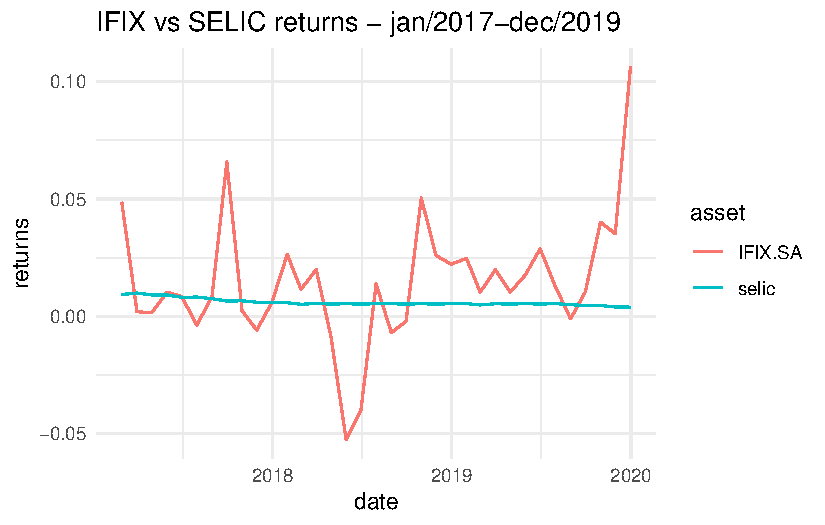
\includegraphics{FII_portfolio_opt_R_files/figure-pdf/Graph_1-1.pdf}

}

\caption{returns compared - ploted using plotly}

\end{figure}

\begin{center}
\textbf{2. OBJECTIVE}
\end{center}

This project aimed to simulate an optimize a FII portfolio considering
the scenario of low brazilian economy basic interest rate and
accelerated real state market growing, focusing on some market
indicators such as:

the covariance and the standard deviation to measure volatility and
risk.

Sharpe index, witch measures the adjusted profitability (\(P_r\)) for
the total portfolio risk (\(\sigma\)) , compared with a minimum accepted
return (\(M_r\)).

\[ SI=\frac{\overline{P_r}-M_r}{\sigma_{p}} \]

\(\beta\), witch measures the portfolio sensibility to an specified
market, in this case the IFIX was used as
reference.\[\beta=\frac{Cov(P;IFIX)}{\sigma_{IFIX}^2}\]

\begin{center}
\textbf{3. METODOLOGY AND CONCLUSION}
\end{center}

This work relied on the use of RStudio and various R packages to
manipulate and understand the data, including: Tydiverse(Wickham et al.
2019) ,Lubridade(Grolemund and Wickham 2011)for general data
manipulation, plotly(Sievert, n.d.) and ggplot2(Wickham 2016) for data
visualization and quantmode(Ryan et al. 2022a), tidyquant(Dancho and
Vaughan 2022) and PerformanceAnalitycs(Peterson et al. 2020) for
financial data vesting, manipulation and computation.

For the assets selection some assumptions were made. Using a filter tool
from the website Clube do FII(ClubeFII, n.d.), all assets with the IPO
(Inicial public offering) prior the year of 2017 and mean monthly
liquidity greater than R\$ 2,000.00 were selected.

The chosen assets price data was downloaded within the time window of
2017 to 2019 with the package quantmod(Ryan et al. 2022b) and Yahoo
Finance({``Yahoo Finance,''} n.d.) as source. After the price data
vesting, followed the monthly log returns calculation using
dplyr(Wickham et al. 2022) and xts(Ryan et al. 2020) to transform the
daily returns in monthly returns. All funds with inconsistent data and
no participation on the market index (IFIX) were discarded at this phase
and 24 assets were selected at the end.

A sample weight vector was created to start the simulations and
optimization with the selected portfolio, the optimization itself was
made adapting a script from codingfinance.com({``Coding Finance''} 2018)
and was achieved calculating the portfolio returns using weights
generated with the base function runif(R Core Team 2022)witch uses
uniform distribution. Folowind this step the market indicators were
calculated and filtered to view the tangent portfolio and the minimum
variance portfolio.

\hypertarget{references}{%
\subsection{References}\label{references}}

\newcounter{foo}
\renewenvironment{CSLReferences}[2] % #1 hanging-ident, #2 entry spacing
 {% don't indent paragraphs
  \setlength{\parindent}{0pt}
  % turn on hanging indent if param 1 is 1
  \ifodd #1 \everypar{\stepcounter{foo}\thefoo.~\setlength{\hangindent}{\cslhangindent}}\ignorespaces\else\everypar{\stepcounter{foo}\thefoo.~}\fi
  % set entry spacing
  \ifnum #2 > 0
  \setlength{\parskip}{#2\baselineskip}
  \fi
 }%
 {}

\hypertarget{refs}{}
\begin{CSLReferences}{1}{0}
\leavevmode\vadjust pre{\hypertarget{ref-clubefii}{}}%
ClubeFII. n.d. {``Clube FII - O maior site de Fundos Imobiliários do
Brasil.''} \url{https://www.clubefii.com.br}.

\leavevmode\vadjust pre{\hypertarget{ref-codingf2018}{}}%
{``Coding Finance.''} 2018.
\url{https://www.codingfinance.com/post/2018-05-31-portfolio-opt-in-r/}.

\leavevmode\vadjust pre{\hypertarget{ref-dancho2022}{}}%
Dancho, Matt, and Davis Vaughan. 2022. \emph{Tidyquant: Tidy
Quantitative Financial Analysis}.
\url{https://CRAN.R-project.org/package=tidyquant}.

\leavevmode\vadjust pre{\hypertarget{ref-grolemund2011}{}}%
Grolemund, Garrett, and Hadley Wickham. 2011. {``Dates and Times Made
Easy with {\textbf{Lubridate}}.''} \emph{Journal of Statistical
Software} 40 (3). \url{https://doi.org/10.18637/jss.v040.i03}.

\leavevmode\vadjust pre{\hypertarget{ref-peterson2020}{}}%
Peterson, Brian G., Peter Carl, Kris Boudt, Ross Bennett, Joshua Ulrich,
Eric Zivot, Dries Cornilly, et al. 2020. \emph{PerformanceAnalytics:
Econometric Tools for Performance and Risk Analysis}.
\url{https://CRAN.R-project.org/package=PerformanceAnalytics}.

\leavevmode\vadjust pre{\hypertarget{ref-rcoreteam2022}{}}%
R Core Team. 2022. {``R: A Language and Environment for Statistical
Computing.''} \url{https://www.r-project.org/}.

\leavevmode\vadjust pre{\hypertarget{ref-ryan2020}{}}%
Ryan, Jeffrey A., Joshua M. Ulrich, Ross Bennett, and Corwin Joy. 2020.
\emph{Xts: eXtensible Time Series}.
\url{https://CRAN.R-project.org/package=xts}.

\leavevmode\vadjust pre{\hypertarget{ref-ryan2022}{}}%
Ryan, Jeffrey A., Joshua M. Ulrich, Ethan B. Smith, Wouter Thielen, Paul
Teetor, and Steve Bronder. 2022a. \emph{Quantmod: Quantitative Financial
Modelling Framework}. \url{https://CRAN.R-project.org/package=quantmod}.

\leavevmode\vadjust pre{\hypertarget{ref-ryan2022a}{}}%
---------. 2022b. \emph{Quantmod: Quantitative Financial Modelling
Framework}. \url{https://CRAN.R-project.org/package=quantmod}.

\leavevmode\vadjust pre{\hypertarget{ref-sievert}{}}%
Sievert, Carson. n.d. \emph{Interactive Web-Based Data Visualization
with r, Plotly, and Shiny}. \url{https://plotly-r.com/}.

\leavevmode\vadjust pre{\hypertarget{ref-wickham2016}{}}%
Wickham, Hadley. 2016. \emph{Ggplot2: Elegant Graphics for Data
Analysis}. New York, NY: Springer Science+Business Media, LLC.

\leavevmode\vadjust pre{\hypertarget{ref-wickham2019}{}}%
Wickham, Hadley, Mara Averick, Jennifer Bryan, Winston Chang, Lucy
McGowan, Romain François, Garrett Grolemund, et al. 2019. {``Welcome to
the Tidyverse.''} \emph{Journal of Open Source Software} 4 (43): 1686.
\url{https://doi.org/10.21105/joss.01686}.

\leavevmode\vadjust pre{\hypertarget{ref-wickham2022}{}}%
Wickham, Hadley, Romain François, Lionel Henry, Kirill Müller, and
RStudio. 2022. \emph{Dplyr: A Grammar of Data Manipulation}.
\url{https://CRAN.R-project.org/package=dplyr}.

\leavevmode\vadjust pre{\hypertarget{ref-yahoofi}{}}%
{``Yahoo Finance.''} n.d. \url{https://finance.yahoo.com/}.

\end{CSLReferences}



\end{document}
